\pagebreak

\hypertarget{tecnologie-informatiche-per-il-web---documentazione-progetto}{%
\section{Tecnologie Informatiche per il Web - Documentazione
Progetto}\label{tecnologie-informatiche-per-il-web---documentazione-progetto}}

\hypertarget{introduzione}{%
\subsection{Introduzione}\label{introduzione}}

Documentazione relativa al progetto ilnale del corso
``\textbf{Tecnologie Informatiche per il Web}'', professore Fraternali
Piero.

Studenti \href{https://github.com/Samdec01}{De Ciechi Samuele} e
\href{https://github.com/SimoneDeidier}{Deidier Simone}, gruppo 9.

Questo file contiene la documentazione relativa sia al progetto
\emph{Pure-HTML} sia al progetto \emph{Rich Internet
Application}.\newline\newline\newline

\emph{Anno Accademico 2022/2023}

\pagebreak

\hypertarget{pure-html}{%
\subsection{\texorpdfstring{\emph{Pure-HTML}}{Pure-HTML}}\label{pure-html}}

\hypertarget{specifica}{%
\subsubsection{Specifica}\label{specifica}}

Un'applicazione permette all'utente (\emph{ad esempio il responsabile
dei servizi ambientali di una regione}) di gestire una collezione di
immagini satellitari e una tassonomia di classificazione utile per
etichettare immagini allo scopo di consentire la ricerca per categoria.
Dopo il login, l'utente accede a una pagina \emph{HOME} in cui compare
un albero gerarchico di categorie. Le categorie non dipendono
dall'utente e sono in comune tra tutti gli utenti.

L'utente può inserire una nuova categoria nell'albero. Per fare ciò usa
una form nella pagina \emph{HOME} in cui specifica il nome della nuova
categoria e sceglie la categoria padre. L'invio della nuova categoria
comporta l'aggiornamento dell'albero: la nuova categoria è appesa alla
categoria padre come ultimo sottoelemento. Alla nuova categoria viene
assegnato un codice numerico che ne riflette la posizione. Dopo la
creazione di una categoria, la pagina \emph{HOME} mostra l'albero
aggiornato. Per velocizzare la costruzione della tassonomia l'utente può
copiare un intero sottoalbero in una data posizione: per fare ciò clicca
sul link ``\emph{copia}'' associato alla categoria radice del
sottoalbero da copiare. A seguito di tale azione l'applicazione mostra,
sempre nella \emph{HOME} page, l'albero con evidenziato il sottoalbero
da copiare: tutte le altre categorie hanno un link ``\emph{copia qui}''.
La selezione di un link ``\emph{copia qui}'' comporta l'inserimento di
una copia del sottoalbero come ultimo figlio della categoria
destinazione.

Per semplicità si ipotizzi che per ogni categoria il numero massimo di
sottocategorie sia 9, numerate da 1 a 9. In questo caso l'operazione di
copia deve controllare che lo spostamento non determini un numero di
sottocategorie superiore a 9. Si preveda anche un link ``\emph{copia
qui}'' non associato a un nodo della tassonomia che permette di copiare
un sotto-albero al primo livello della tassonomia (\emph{se non esistono
già 9 nodi al primo livello della tassonomia}).

\pagebreak

\hypertarget{analisi-della-specifica}{%
\subsubsection{Analisi della specifica}\label{analisi-della-specifica}}

\hypertarget{analisi-del-testo-per-la-creazione-del-database}{%
\paragraph{Analisi del testo per la creazione del
database}\label{analisi-del-testo-per-la-creazione-del-database}}

Un'applicazione permette all'\textbf{utente} di gestire una collezione
di immagini satellitari e una tassonomia di classificazione utile per
etichettare immagini allo scopo di consentire la ricerca per categoria.
Dopo il login (\(\implies\) \emph{username e password}), l'utente accede
a una pagina HOME in cui compare un albero gerarchico di
\textbf{categorie}. \textbf{\emph{Le categorie non dipendono dall'utente
e sono in comune tra tutti gli utenti}}.

L'utente può inserire una nuova categoria nell'albero. Per fare ciò usa
una form nella pagina HOME in cui specifica il nome della nuova
categoria e sceglie la \emph{categoria padre}. L'invio della nuova
categoria comporta l'aggiornamento dell'albero: la nuova categoria è
appesa alla categoria padre come ultimo sottoelemento. Alla nuova
categoria viene assegnato un \emph{codice numerico} che ne riflette la
posizione\ldots{}

\begin{figure}
\centering
\includegraphics{../../../../_resources/diagrammaER.png}
\caption{\emph{Diagramma E-R del database utilizzato}}
\end{figure}

\pagebreak

\hypertarget{creazione-del-database-in-mysqlworkbench}{%
\paragraph{Creazione del database in
MySQLWorkbench}\label{creazione-del-database-in-mysqlworkbench}}

\begin{Shaded}
\begin{Highlighting}[]
\KeywordTok{CREATE} \KeywordTok{TABLE} \KeywordTok{Category}\NormalTok{ (}
\NormalTok{  categoryID bigint }\KeywordTok{NOT} \KeywordTok{NULL}\NormalTok{,}
\NormalTok{  name }\DataTypeTok{varchar}\NormalTok{(}\DecValTok{45}\NormalTok{) }\KeywordTok{NOT} \KeywordTok{NULL}\NormalTok{,}
\NormalTok{  parentID bigint }\KeywordTok{DEFAULT} \KeywordTok{NULL}\NormalTok{,}
  \KeywordTok{PRIMARY} \KeywordTok{KEY}\NormalTok{ (categoryID),}
  \KeywordTok{FOREIGN} \KeywordTok{KEY}\NormalTok{ (parentID) }\KeywordTok{REFERENCES} \KeywordTok{Category}\NormalTok{ (categoryID)}
  \KeywordTok{ON} \KeywordTok{UPDATE} \KeywordTok{CASCADE} \KeywordTok{ON} \KeywordTok{DELETE} \KeywordTok{NO}\NormalTok{ ACTION}
\NormalTok{)}

\KeywordTok{CREATE} \KeywordTok{TABLE} \FunctionTok{User}\NormalTok{ (}
\NormalTok{  username }\DataTypeTok{varchar}\NormalTok{(}\DecValTok{45}\NormalTok{) }\KeywordTok{NOT} \KeywordTok{NULL}\NormalTok{,}
  \KeywordTok{password} \DataTypeTok{varchar}\NormalTok{(}\DecValTok{45}\NormalTok{) }\KeywordTok{NOT} \KeywordTok{NULL}\NormalTok{,}
  \KeywordTok{PRIMARY} \KeywordTok{KEY}\NormalTok{ (username)}
\NormalTok{) }
\end{Highlighting}
\end{Shaded}

\hypertarget{note-relative-alla-progettazione-del-database}{%
\paragraph{Note relative alla progettazione del
database}\label{note-relative-alla-progettazione-del-database}}

Abbiamo deciso di utilizzare \emph{bigint} per \emph{categoryID} e
\emph{parentID} così da permettere una maggiore libertà agli utenti nel
creare diversi annidamenti di categorie, rispetto alla quantità di
sottocategorie che avrebbero potuto creare con un semplice \emph{int}.

Abbiamo inoltre scelto di non mettere una tabella intermedia fra le due
categorie. Questo è dovuto al fatto che tutti gli utenti possono vedere
tutte le categorie e quindi non c'è motivo di tenere traccia di chi crea
una categoria o di dare visibilità ad alcune categorie a solo alcuni
utenti.

\pagebreak

\hypertarget{analisi-dei-requisiti-dellapplicazione}{%
\subsubsection{Analisi dei requisiti
dell'applicazione}\label{analisi-dei-requisiti-dellapplicazione}}

Un'applicazione permette all'utente (ad esempio il responsabile dei
servizi ambientali di una regione) di gestire una collezione di immagini
satellitari e una tassonomia di classificazione utile per etichettare
immagini allo scopo di consentire la ricerca per categoria. \emph{Dopo
il login}, \textbf{\emph{l'utente accede a una pagina}} HOME in cui
compare un \textbf{albero gerarchico di categorie.} Le categorie non
dipendono dall'utente e sono in comune tra tutti gli utenti.

L'utente può inserire una nuova categoria nell'albero. Per fare ciò usa
\textbf{una form} nella pagina HOME in cui specifica il nome della nuova
categoria e sceglie la categoria padre. \textbf{\emph{L'invio della
nuova categoria}} comporta l'aggiornamento dell'albero: \emph{la nuova
categoria è appesa alla categoria padre come ultimo sottoelemento}. Alla
nuova categoria viene assegnato un codice numerico che ne riflette la
posizione. Dopo la creazione di una categoria, la pagina HOME mostra
l'albero aggiornato. Per velocizzare la costruzione della tassonomia
l'utente può copiare un intero sottoalbero in una data posizione: per
fare ciò \textbf{\emph{clicca sul link}} ``\textbf{copia}'' associato
alla categoria radice del sottoalbero da copiare. A seguito di tale
azione l'applicazione mostra, sempre nella HOME page, l'albero con
evidenziato il sottoalbero da copiare: tutte le altre categorie hanno un
link ``\textbf{copia qui}'' \emph{\textbf{La selezione di un link
``copia qui''} comporta l'inserimento di una copia del sottoalbero come
ultimo figlio della categoria destinazione}.

Per semplicità si ipotizzi che per ogni categoria il numero massimo di
sottocategorie sia 9, numerate da 1 a 9. In questo caso l'operazione di
copia deve controllare che lo spostamento non determini un numero di
sottocategorie superiore a 9. Si preveda anche un \textbf{link ``copia
qui'' non associato a un nodo della tassonomia} \emph{che permette di
copiare un sotto-albero al primo livello della tassonomia} (se non
esistono già 9 nodi al primo livello della tassonomia).

\begin{itemize}
\tightlist
\item
  \textbf{Pages} (\emph{views}): pagina di login, pagina HOME.
\end{itemize}

\begin{longtable}[]{@{}ccc@{}}
\toprule()
View components & Events & Action \\
\midrule()
\endhead
\textbf{Grassetto} & \textbf{\emph{Grassetto e corsivo}} &
\emph{Corsivo} \\
\bottomrule()
\end{longtable}

\pagebreak

\hypertarget{design-dellapplicazione}{%
\subsubsection{Design dell'applicazione}\label{design-dellapplicazione}}

\begin{figure}
\centering
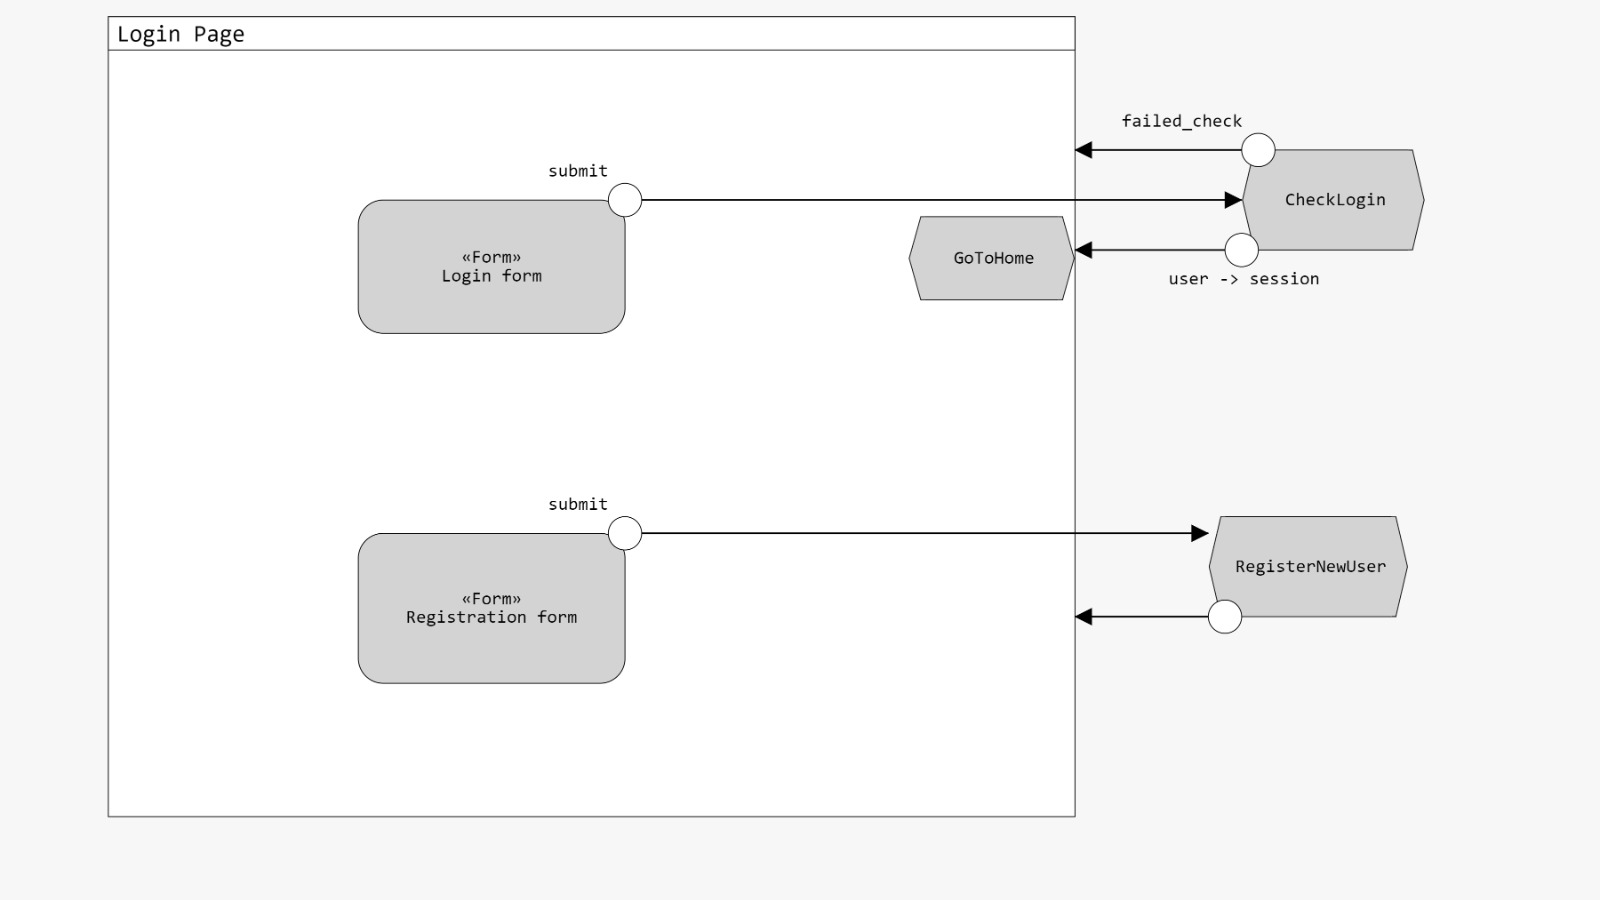
\includegraphics{../../../../_resources/IFML - login.jpeg}
\caption{\emph{Diagramma IFML della pagina LOGIN.}}
\end{figure}

\pagebreak

\begin{figure}
\centering
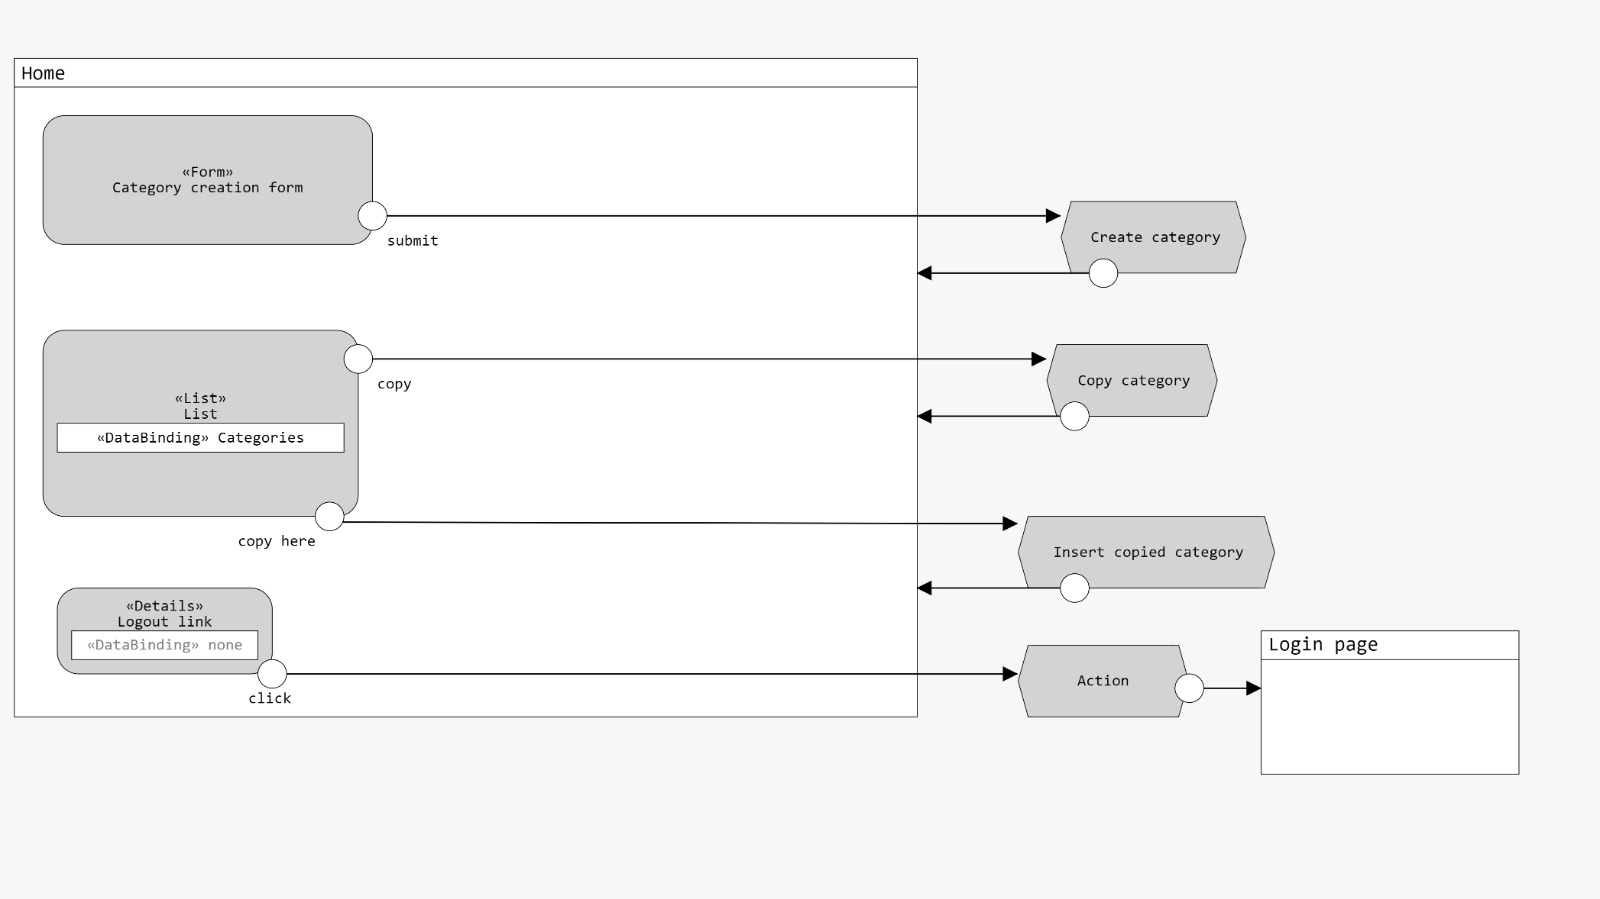
\includegraphics{../../../../_resources/IFML - HOME - pure-html.jpeg}
\caption{\emph{Diagramma IFML della pagina HOME.}}
\end{figure}

\pagebreak

\hypertarget{componenti}{%
\paragraph{Componenti}\label{componenti}}

\begin{itemize}
\tightlist
\item
  Model Objects (\emph{Beans}):

  \begin{itemize}
  \tightlist
  \item
    User
  \item
    Category
  \end{itemize}
\item
  Data Access Objects (\emph{Classes}):

  \begin{itemize}
  \tightlist
  \item
    UserDAO

    \begin{itemize}
    \tightlist
    \item
      checkLogin(username, password)
    \item
      registerNewUser(username, password)
    \end{itemize}
  \item
    CategoriesDAO

    \begin{itemize}
    \tightlist
    \item
      findAllCategories()
    \item
      createCategory(name, parentID)
    \item
      findLastChildrenID(categoryList, parentID)
    \item
      checkExistingCategoryFromID(categoryID)
    \item
      findSubCategories(categoryID)
    \item
      toCopyList(categoryID)
    \item
      insertCopiedCategory(categoryID, parentID)
    \item
      addCategoryInDatabase(newID, name, newParentID)
    \item
      orderCategoriesList(unorderedList, parentID)
    \end{itemize}
  \end{itemize}
\item
  Controllers (\emph{Servlets}):

  \begin{itemize}
  \tightlist
  \item
    GoToHome
  \item
    CheckLogin
  \item
    Logout
  \item
    CreateCategory
  \item
    CopyCategory
  \item
    InsertCopiedCategory
  \end{itemize}
\item
  Filters:

  \begin{itemize}
  \tightlist
  \item
    NoCacheFilter
  \item
    UserChecker
  \end{itemize}
\item
  View (\emph{Templates}):

  \begin{itemize}
  \tightlist
  \item
    Login page (\emph{index.html})
  \item
    Home
  \end{itemize}
\end{itemize}

\pagebreak

\hypertarget{sequence-diagrams-evento-login}{%
\subsubsection{\texorpdfstring{\emph{Sequence Diagrams}: Evento
Login}{Sequence Diagrams: Evento Login}}\label{sequence-diagrams-evento-login}}

\begin{figure}
\centering
\includegraphics{../../../../_resources/Event_Login-1.png}
\caption{\emph{Sequence diagram dell'evento Login.}}
\end{figure}

\pagebreak

\hypertarget{sequence-diagrams-evento-registernewuser}{%
\subsubsection{\texorpdfstring{\emph{Sequence Diagrams}: Evento
RegisterNewUser}{Sequence Diagrams: Evento RegisterNewUser}}\label{sequence-diagrams-evento-registernewuser}}

\begin{figure}
\centering
\includegraphics{../../../../_resources/Event_Register_New_User-1.png}
\caption{\emph{Sequence diagram dell'evento RegisterNewUser.}}
\end{figure}

\pagebreak

\hypertarget{sequence-diagrams-evento-gotohome}{%
\subsubsection{\texorpdfstring{\emph{Sequence Diagrams}: Evento
GoToHome}{Sequence Diagrams: Evento GoToHome}}\label{sequence-diagrams-evento-gotohome}}

\begin{figure}
\centering
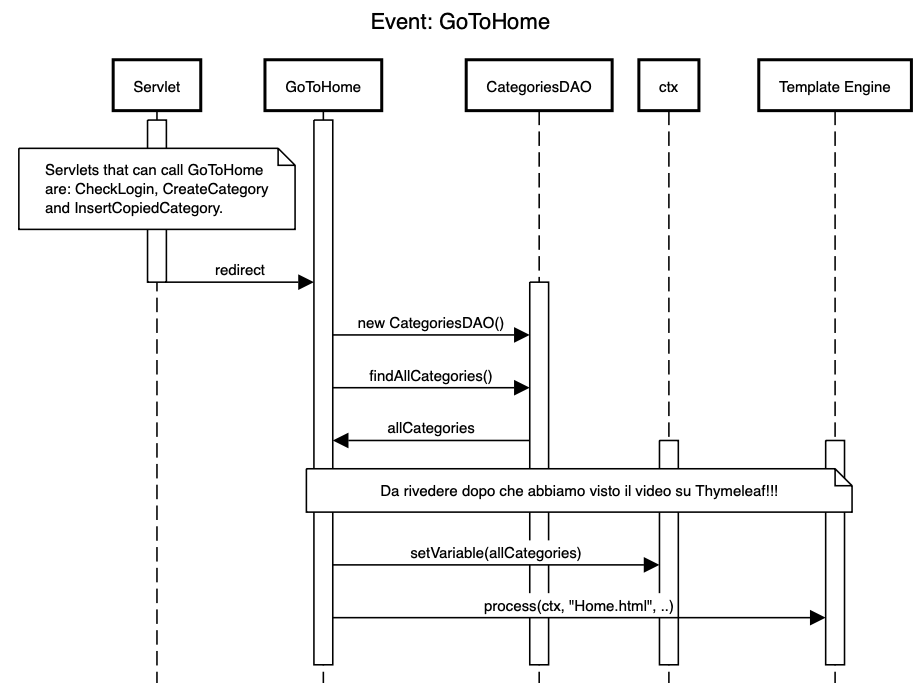
\includegraphics{../../../../_resources/Event_GoToHome.png}
\caption{\emph{Sequence diagram dell'evento GoToHome.}}
\end{figure}

\pagebreak

\hypertarget{sequence-diagrams-evento-createcategory}{%
\subsubsection{\texorpdfstring{\emph{Sequence Diagrams}: Evento
CreateCategory}{Sequence Diagrams: Evento CreateCategory}}\label{sequence-diagrams-evento-createcategory}}

\begin{figure}
\centering
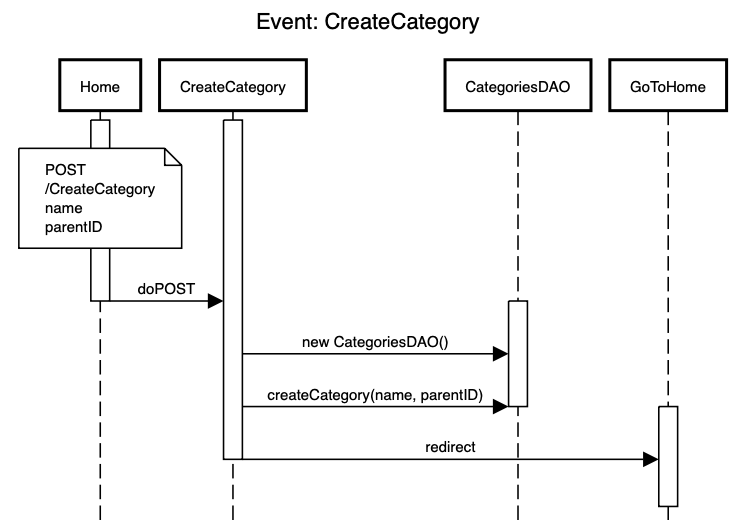
\includegraphics{../../../../_resources/Event_CreateCategory.png}
\caption{\emph{Sequence diagram dell'evento CreateCategory.}}
\end{figure}

\pagebreak

\hypertarget{sequence-diagrams-evento-copycategory}{%
\subsubsection{\texorpdfstring{\emph{Sequence Diagrams}: Evento
CopyCategory}{Sequence Diagrams: Evento CopyCategory}}\label{sequence-diagrams-evento-copycategory}}

\begin{figure}
\centering
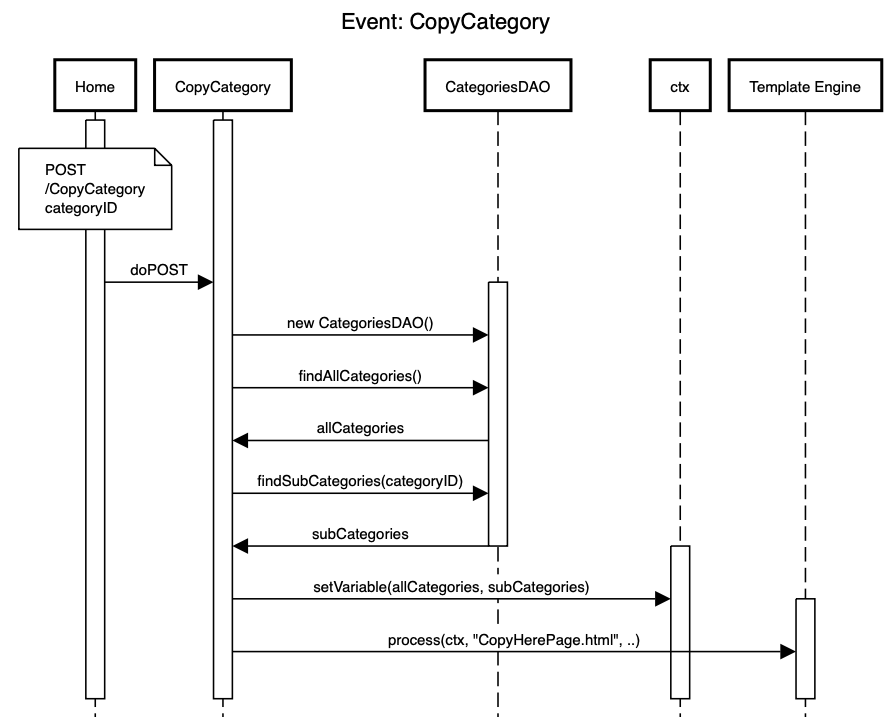
\includegraphics{../../../../_resources/Event_CopyCategory.png}
\caption{\emph{Sequence diagram dell'evento CopyCategory.}}
\end{figure}

\pagebreak

\hypertarget{sequence-diagrams-evento-insertcopiedcategory}{%
\subsubsection{\texorpdfstring{\emph{Sequence Diagrams}: Evento
InsertCopiedCategory}{Sequence Diagrams: Evento InsertCopiedCategory}}\label{sequence-diagrams-evento-insertcopiedcategory}}

\begin{figure}
\centering
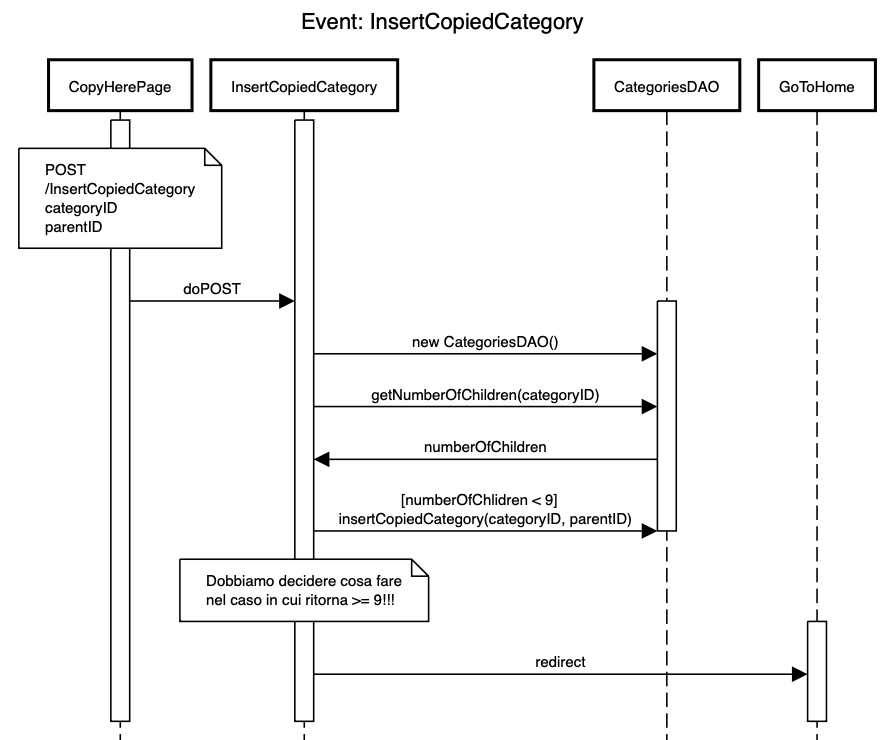
\includegraphics{../../../../_resources/Event_InsertCopiedCategory.png}
\caption{\emph{Sequence diagram dell'evento InsertCopiedCategory.}}
\end{figure}

\pagebreak

\hypertarget{sequence-diagrams-evento-logout}{%
\subsubsection{\texorpdfstring{\emph{Sequence Diagrams}: Evento
Logout}{Sequence Diagrams: Evento Logout}}\label{sequence-diagrams-evento-logout}}

\begin{figure}
\centering
\includegraphics{../../../../_resources/Event_Logout-1.png}
\caption{\emph{Sequence diagram dell'evento Logout.}}
\end{figure}

\pagebreak

\hypertarget{rich-internet-application}{%
\subsection{\texorpdfstring{\emph{Rich Internet
Application}}{Rich Internet Application}}\label{rich-internet-application}}

\hypertarget{completamento-della-specifica}{%
\subsubsection{Completamento della
specifica}\label{completamento-della-specifica}}

Si realizzi un'applicazione client server web che estende e/o modifica
le specifiche precedenti come segue:

\begin{itemize}
\tightlist
\item
  Dopo il login dell'utente, l'intera applicazione è realizzata con
  un'unica pagina.
\item
  Ogni interazione dell'utente è gestita senza ricaricare completamente
  la pagina, ma produce l'invocazione asincrona del server e l'eventuale
  modifica del contenuto da aggiornare a seguito dell'evento.
\item
  La funzione di copia di un sottoalbero è realizzata mediante
  \emph{drag \& drop}. A seguito del drop della radice del sottoalbero
  da copiare compare una finestra di dialogo con cui l'utente può
  confermare o cancellare la copia. La conferma produce l'aggiornamento
  solo a lato client dell'albero. La cancellazione riconduce allo stato
  precedente al \emph{drag \& drop}. A seguito della conferma compare un
  bottone \emph{SALVA} che consente il salvataggio a lato server della
  tassonomia modificata.
\item
  L'utente può cliccare sul nome di una categoria. A seguito di tale
  evento compare al posto del nome un campo di input contente la stringa
  del nome modificabile. L'evento di perdita del focus del campo di
  input produce il salvataggio nel database del nome modificato della
  categoria.
\end{itemize}

\pagebreak

\hypertarget{design-dellapplicazione-1}{%
\subsubsection{Design
dell'applicazione}\label{design-dellapplicazione-1}}

\begin{figure}
\centering
\includegraphics{../../../../_resources/PHOTO-2023-06-25-19-11-05.jpg}
\caption{\emph{Diagramma IFML della pagina HOME - versione RIA.}}
\end{figure}

\pagebreak

\hypertarget{eventi-ed-azioni}{%
\subsubsection{Eventi ed Azioni}\label{eventi-ed-azioni}}

\begin{figure}
\centering
\includegraphics{../../../../_resources/Screenshot 2023-06-27 alle 00.20.30.png}
\caption{\emph{Tabella degli Eventi e delle Azioni.}}
\end{figure}

\pagebreak

\hypertarget{controller---event-handler}{%
\subsubsection{\texorpdfstring{Controller - \emph{Event
Handler}}{Controller - Event Handler}}\label{controller---event-handler}}

\begin{figure}
\centering
\includegraphics{../../../../_resources/Screenshot 2023-06-27 alle 00.18.00.png}
\caption{\emph{Tabella del Controller - Event Handler.}}
\end{figure}

\pagebreak

\hypertarget{event-e-view-dynamics}{%
\subsubsection{\texorpdfstring{\emph{Event} e \emph{View
Dynamics}}{Event e View Dynamics}}\label{event-e-view-dynamics}}

\begin{figure}
\centering
\includegraphics{../../../../_resources/Screenshot 2023-06-27 alle 00.24.23.png}
\caption{\emph{Event \& View Dynamics.}}
\end{figure}

\pagebreak

\hypertarget{dao-e-model-objects---server-side}{%
\paragraph{\texorpdfstring{DAO e \emph{Model Objects} - server
side}{DAO e Model Objects - server side}}\label{dao-e-model-objects---server-side}}

\begin{itemize}
\tightlist
\item
  Controllers (\emph{Servlets}):

  \begin{itemize}
  \tightlist
  \item
    CheckLogin
  \item
    Logout
  \item
    CreateCategory
  \item
    InsertCopiedCategory
  \item
    GetCategories
  \item
    RegisterNewUser
  \item
    ChangeCategoryName
  \end{itemize}
\item
  Filters:

  \begin{itemize}
  \tightlist
  \item
    NoCacheFilter
  \item
    UserChecker
  \end{itemize}
\item
  Model Objects (\emph{Beans}):

  \begin{itemize}
  \tightlist
  \item
    User
  \item
    Category
  \end{itemize}
\item
  Data Access Objects (\emph{Classes}):

  \begin{itemize}
  \tightlist
  \item
    UserDAO

    \begin{itemize}
    \tightlist
    \item
      checkLogin(username, password)
    \item
      registerNewUser(username, password)
    \end{itemize}
  \item
    CategoriesDAO

    \begin{itemize}
    \tightlist
    \item
      findAllCategories()
    \item
      createCategory(name, parentID)
    \item
      findLastChildrenID(categoryList, parentID)
    \item
      insertCopiedCategory(categoryID, parentID)
    \item
      addCategoryInDatabase(newID, name, newParentID)
    \item
      orderCategoriesList(unorderedList, parentID)
    \item
      changeCategoryName(categoryID, newName)
    \end{itemize}
  \end{itemize}
\end{itemize}

\pagebreak

\hypertarget{view-e-view-components---client-side}{%
\subsubsection{\texorpdfstring{\emph{View} e \emph{View Components} -
client
side}{View e View Components - client side}}\label{view-e-view-components---client-side}}

\emph{index.html + loginPage.js}:

\begin{itemize}
\tightlist
\item
  Login form \(\implies\) gestione \emph{evento submit} per effettuare
  il login e gli eventuali errori.
\item
  Registration form \(\implies\) gestione \emph{evento submit} per
  registrare un nuovo utente ed eventuali errori.
\end{itemize}

\emph{home.html + home.js}:

\begin{itemize}
\tightlist
\item
  CategoriesContainer

  \begin{itemize}
  \tightlist
  \item
    \emph{update()} \(\implies\) richiede al server la lista di
    categorie nel database.
  \item
    \emph{orderList()} \(\implies\) riordina per la visualizzazione una
    lista di cateogire non ordinata.
  \item
    \emph{createCategoriesHTML()} \(\implies\) crea gli elementi HTML
    per la visualizzazione delle categorie, registra tutti gli eventi
    dei componenti HTML (\emph{drag\&drop, cambio del nome con il
    click}).
  \item
    \emph{showTemporaryList()} \(\implies\) aggiorna a schermo la lista
    di categorie \textbf{dopo l'evento drag\&drop} e gestisce anche la
    creazione del \emph{button} per salvare le modifiche al database.
  \item
    \emph{getListOfNewCategories()} \(\implies\) calcola gli \emph{ID}
    degli elementi copiati tramite funzione \emph{drag\&drop}, gestendo
    eventuali errori.
  \item
    \emph{findLastChildrenID()} \(\implies\) restituisce l'ID
    dell'ultimo figlio dato un nodo padre.
  \end{itemize}
\item
  CreateCategoryForm

  \begin{itemize}
  \tightlist
  \item
    \emph{setEvent()} \(\implies\) registra l'evento relativo al
    \emph{button} del form.
  \item
    \emph{refresh()} \(\implies\) riaggiorna le opzioni disponibili nel
    form per la creazione di una nuova categoria scegliendo la categoria
    padre.
  \end{itemize}
\item
  LogoutManager

  \begin{itemize}
  \tightlist
  \item
    \emph{setEvent()} \(\implies\) registra l'evento relativo
    all'\emph{anchor} per il logout dal sito.
  \item
    \emph{show()} \(\implies\) imposta la visibilità del messaggio di
    logout.
  \end{itemize}
\end{itemize}

\pagebreak

\hypertarget{sequence-diagrams-evento-login-1}{%
\subsubsection{\texorpdfstring{\emph{Sequence Diagrams}: Evento
Login}{Sequence Diagrams: Evento Login}}\label{sequence-diagrams-evento-login-1}}

\begin{figure}
\centering
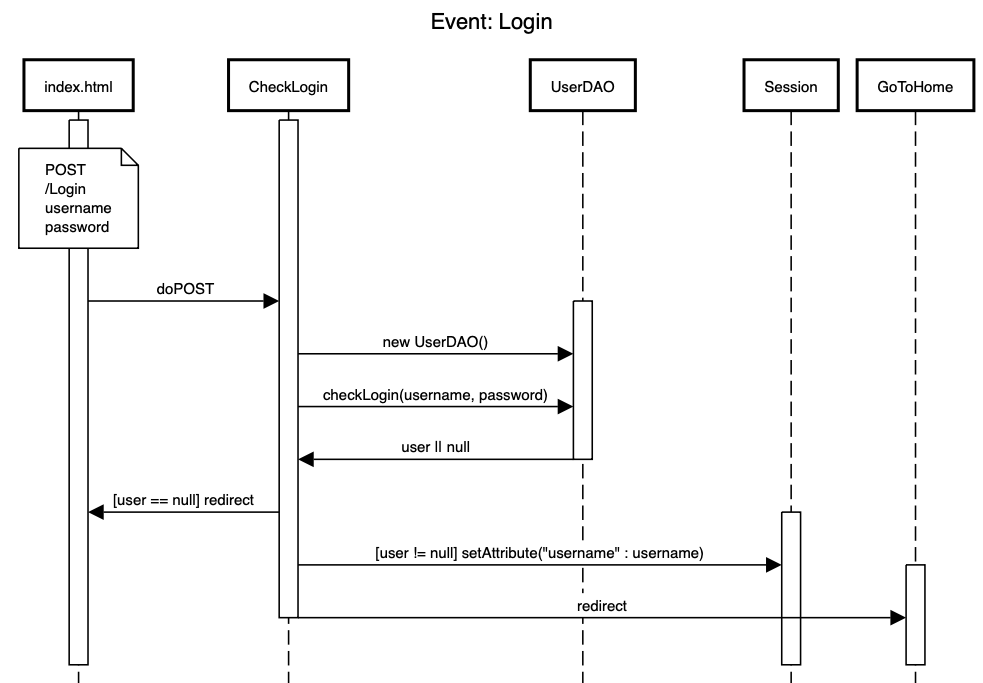
\includegraphics{../../../../_resources/Event_Login.png}
\caption{\emph{Sequence diagram dell'evento Login.}}
\end{figure}

\pagebreak

\hypertarget{sequence-diagrams-evento-register-new-user}{%
\subsubsection{\texorpdfstring{\emph{Sequence Diagrams}: Evento Register
New
User}{Sequence Diagrams: Evento Register New User}}\label{sequence-diagrams-evento-register-new-user}}

\begin{figure}
\centering
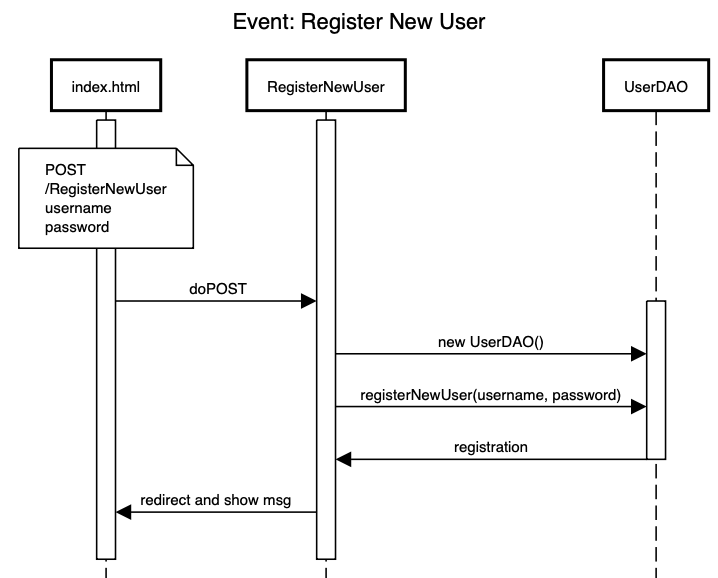
\includegraphics{../../../../_resources/Event_Register_New_User.png}
\caption{\emph{Sequence diagram dell'evento RegisterNewUser.}}
\end{figure}

\pagebreak

\hypertarget{sequence-diagrams-evento-home-load}{%
\subsubsection{\texorpdfstring{\emph{Sequence Diagrams}: Evento Home
load}{Sequence Diagrams: Evento Home load}}\label{sequence-diagrams-evento-home-load}}

\begin{figure}
\centering
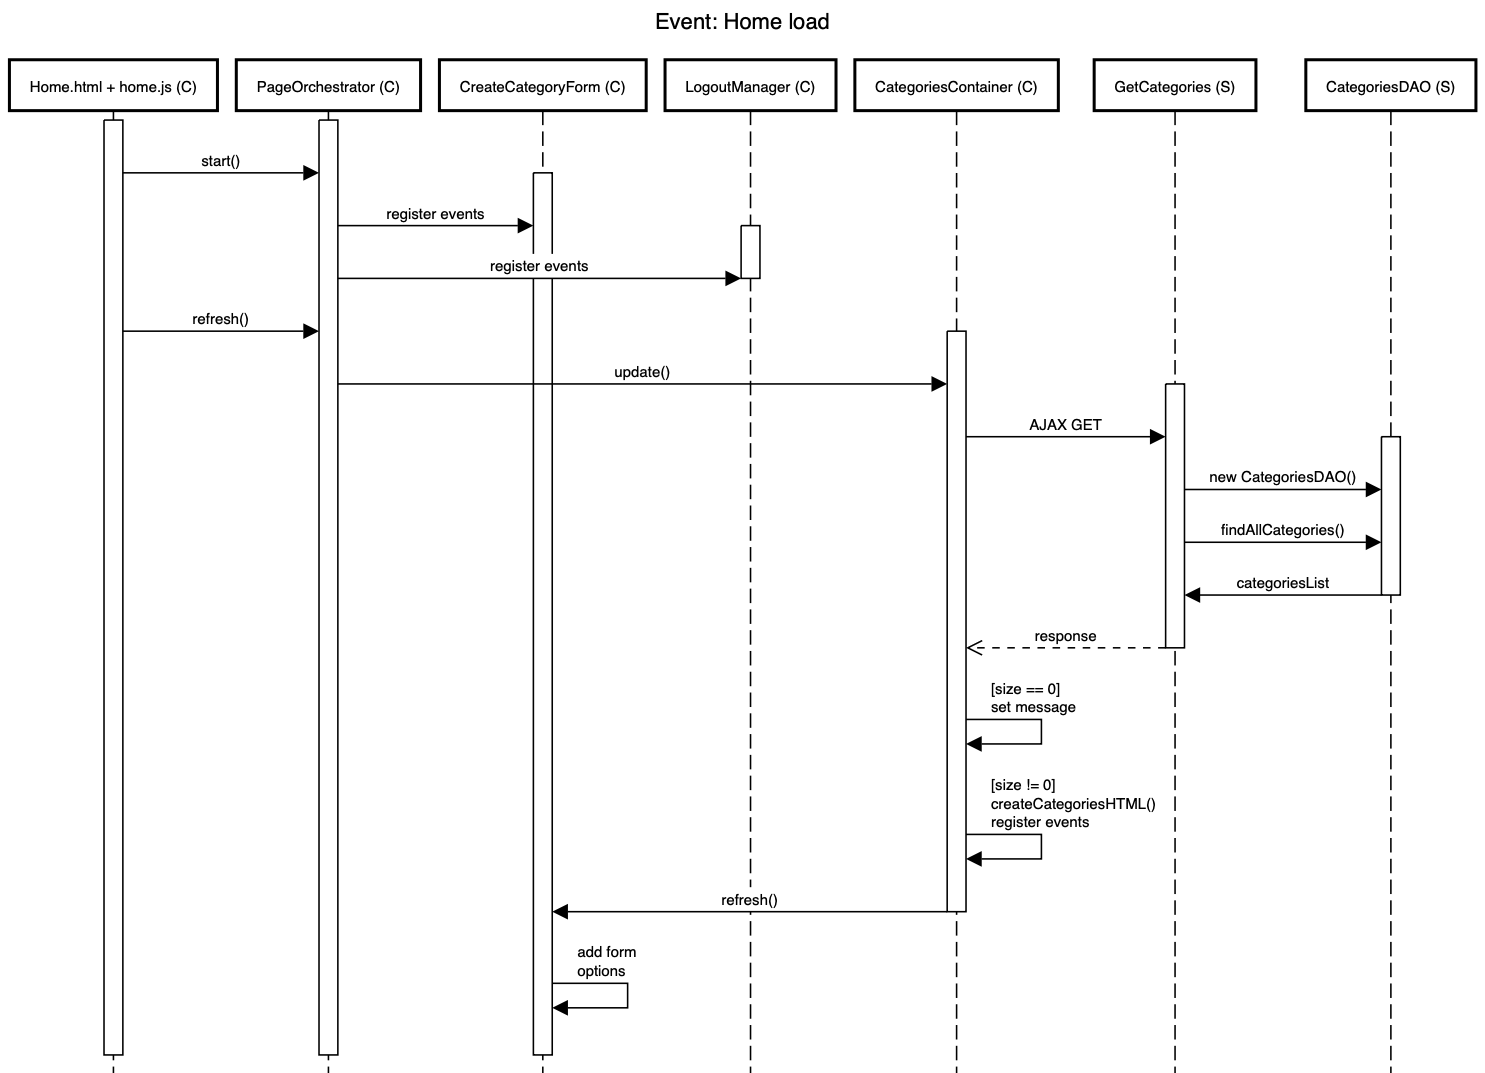
\includegraphics{../../../../_resources/Event_Home_load.png}
\caption{\emph{Sequence diagram dell'evento Home load.}}
\end{figure}

\pagebreak

\hypertarget{sequence-diagrams-evento-create-category}{%
\subsubsection{\texorpdfstring{\emph{Sequence Diagrams}: Evento Create
Category}{Sequence Diagrams: Evento Create Category}}\label{sequence-diagrams-evento-create-category}}

\begin{figure}
\centering
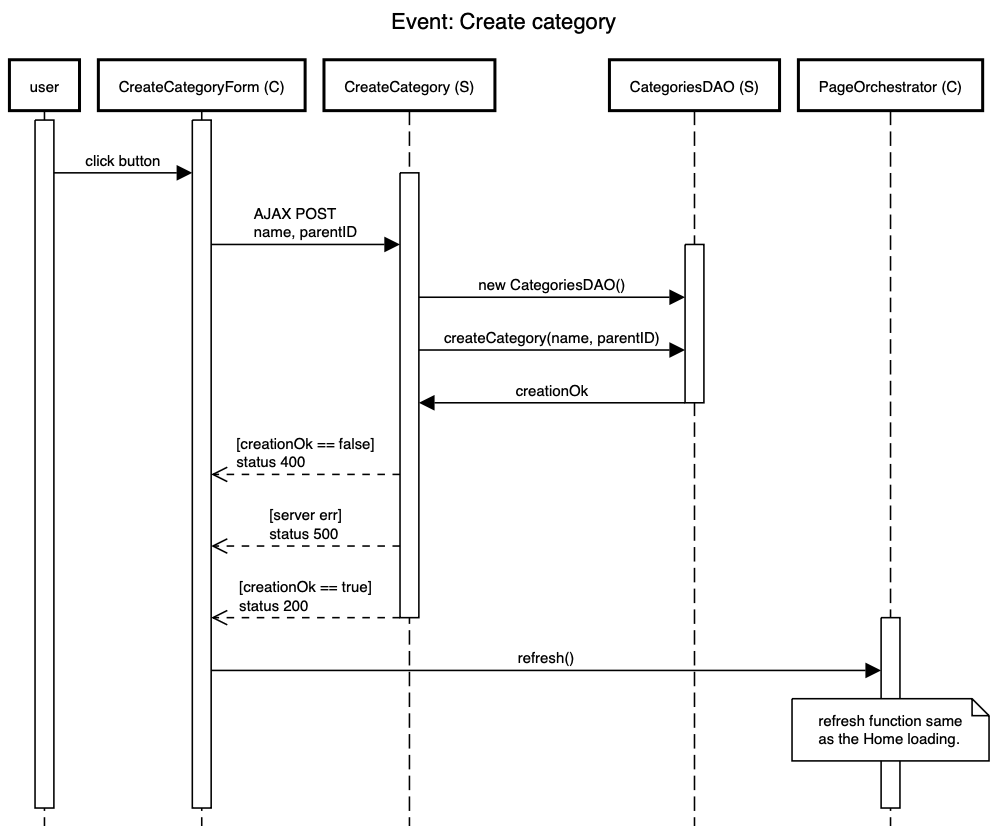
\includegraphics{../../../../_resources/Event_Create_Category.png}
\caption{\emph{Sequence diagram dell'evento CreateCategory.}}
\end{figure}

\pagebreak

\hypertarget{sequence-diagrams-evento-insert-copied-category}{%
\subsubsection{\texorpdfstring{\emph{Sequence Diagrams}: Evento Insert
Copied
Category}{Sequence Diagrams: Evento Insert Copied Category}}\label{sequence-diagrams-evento-insert-copied-category}}

\begin{figure}
\centering
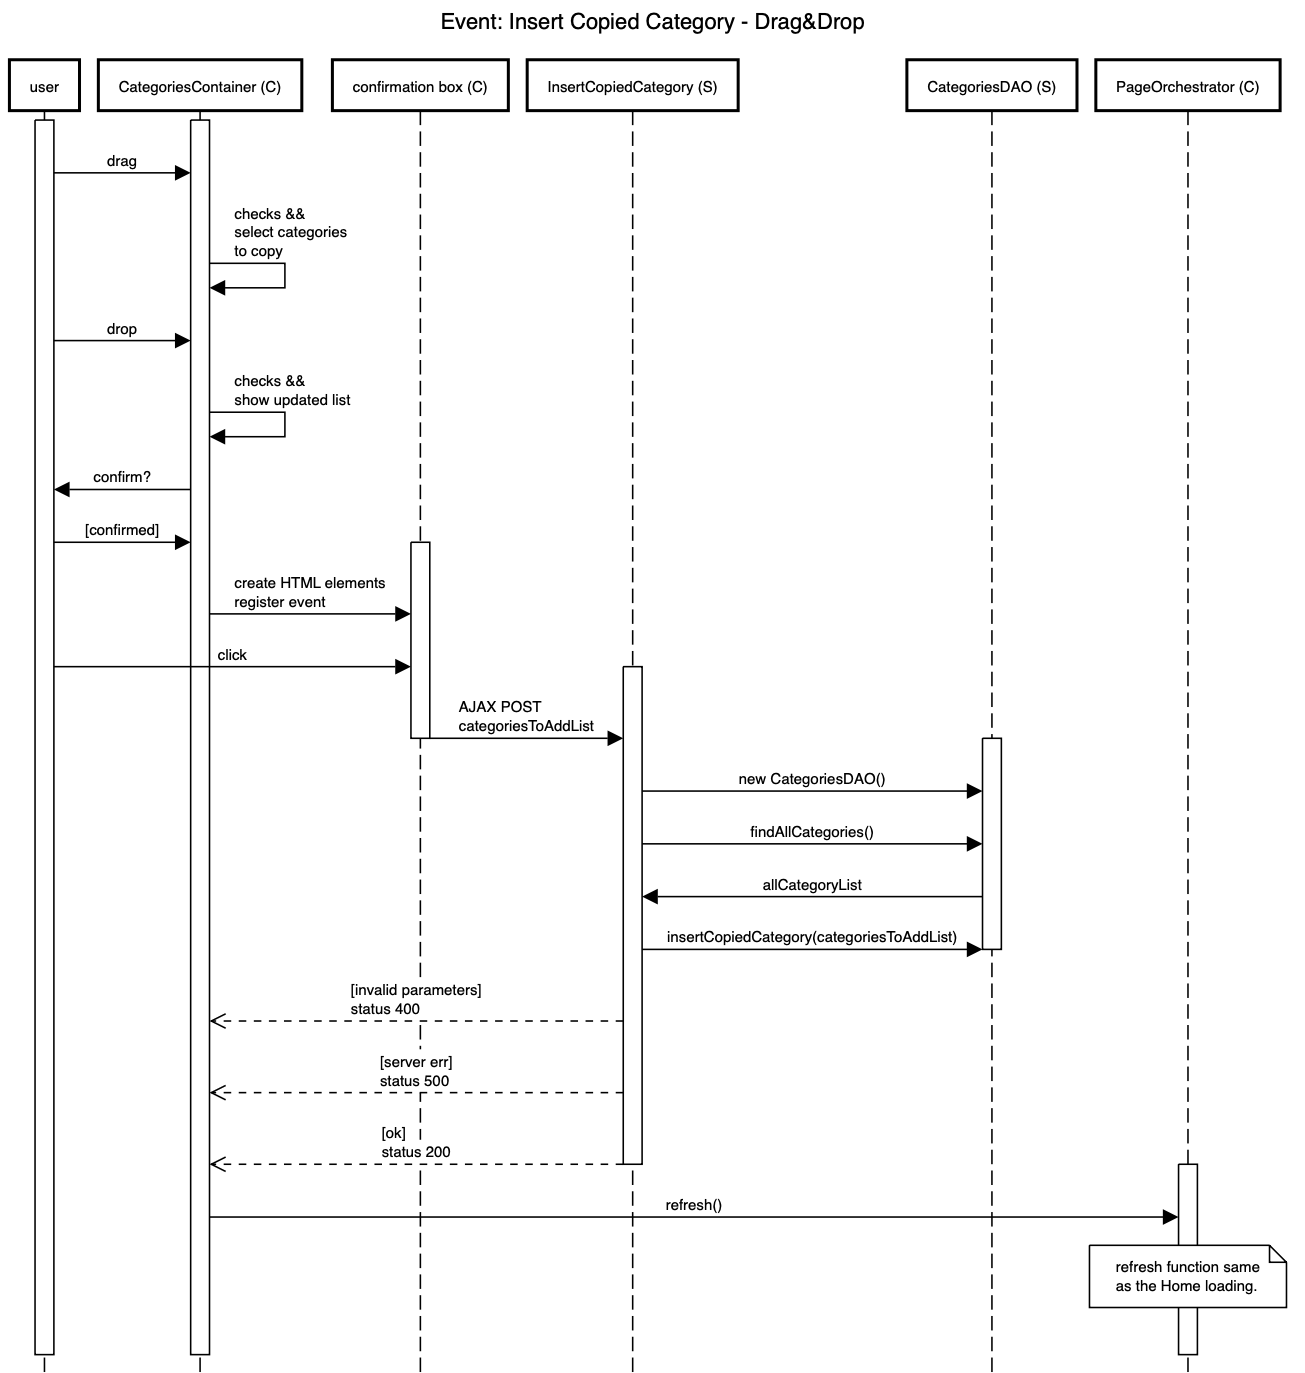
\includegraphics{../../../../_resources/Event_Insert_Copied_Category.png}
\caption{\emph{Sequence diagram dell'evento InsertCopiedCategory.}}
\end{figure}

\pagebreak

\hypertarget{sequence-diagrams-evento-change-category-name}{%
\subsubsection{\texorpdfstring{\emph{Sequence Diagrams}: Evento Change
Category
Name}{Sequence Diagrams: Evento Change Category Name}}\label{sequence-diagrams-evento-change-category-name}}

\begin{figure}
\centering
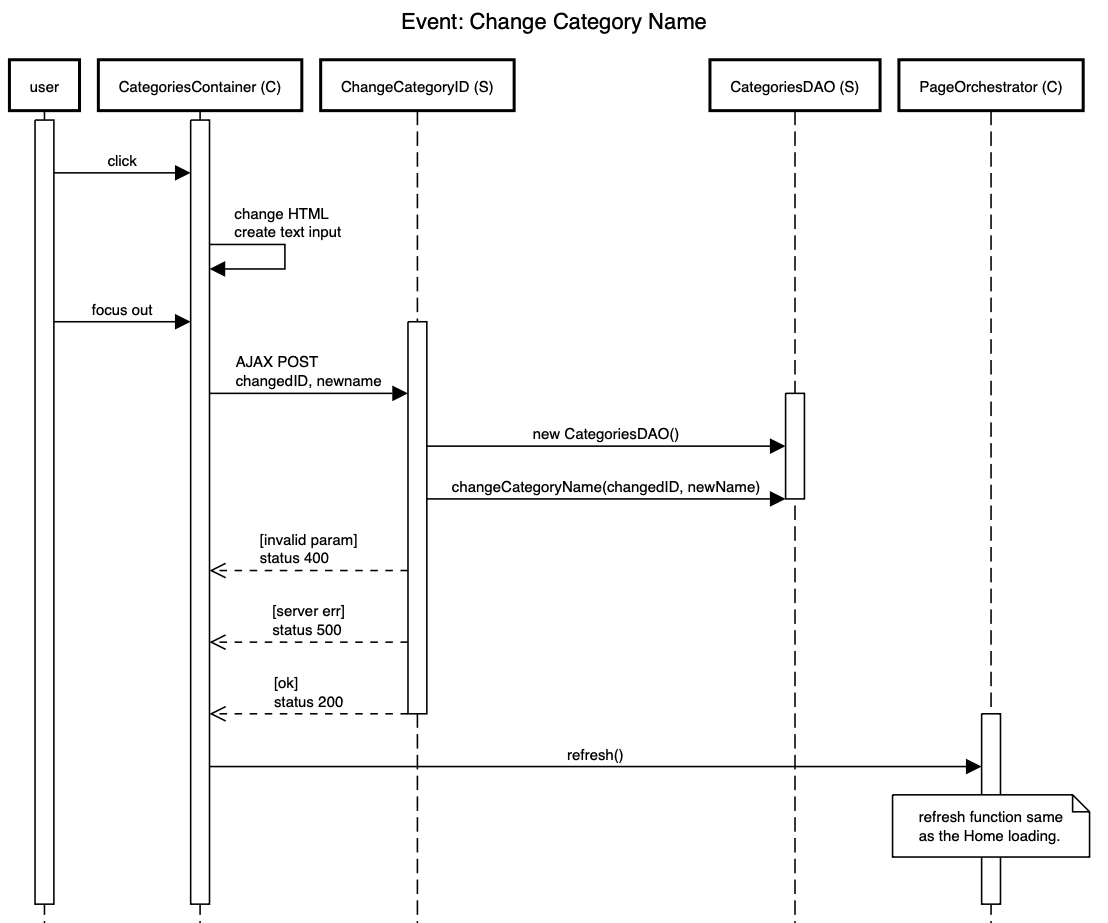
\includegraphics{../../../../_resources/Event_Change_Category_Name.png}
\caption{\emph{Sequence diagram dell'evento ChangeCategoryName.}}
\end{figure}

\pagebreak

\hypertarget{sequence-diagrams-evento-logout-1}{%
\subsubsection{\texorpdfstring{\emph{Sequence Diagrams}: Evento
Logout}{Sequence Diagrams: Evento Logout}}\label{sequence-diagrams-evento-logout-1}}

\begin{figure}
\centering
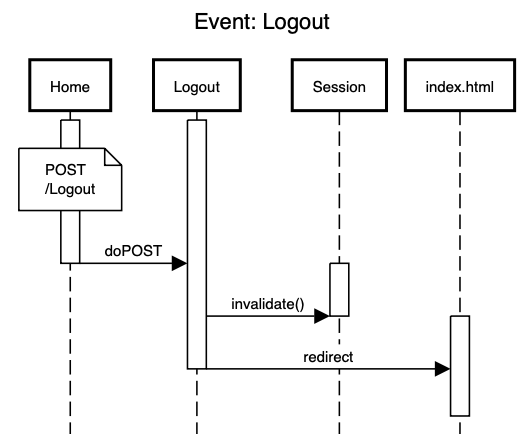
\includegraphics{../../../../_resources/Event_Logout.png}
\caption{\emph{Sequence diagram dell'evento Logout.}}
\end{figure}
